\documentclass[conference]{IEEEtran}

\usepackage{cite}
\usepackage{amsmath}
\usepackage{algorithmic}
\usepackage{url}
\usepackage[utf8]{inputenc}
\usepackage[pdftex]{graphicx}

\hyphenation{}

\begin{document}
\title{Relatório do Trabalho 1\\ de Aprendizado de Máquina}

\author{\IEEEauthorblockN{Fábio Beranizo Fontes Lopes}
\IEEEauthorblockA{Escola de Artes, Ciências e Humanidades (EACH)\\
Universidade de São Paulo (USP)\\
Email: f.lopes@usp.br}}

\maketitle

Este relatório tem como objetivo mostrar os procedimentos e resultados do Trabalho 1 da disciplina de Aprendizado de Máquina. O propósito dessa tarefa foi testar diferentes algoritmos em atividades de reconhecimento biométrico. Duas técnicas de aprendizado supervisionado foram escolhidas para comparação: Multilayer Perceptron (MLP) e Support Vector Machines (SVM).
% Ambos algoritmos foram implementados em Python.

As seções a seguir explicam as atividades de pré-processamento do conjunto de dados, o treinamento dos modelos e uma discussão dos resultados obtidos.

\section{Base de Dados}
A base de dados utilizada neste trabalho foi a Homologous Multi-modal Traits Database da Shandong University (SDUMLA-HMT) \cite{sdumlahtm}. Este conjunto de dados contém faces de 106 indivíduos em 7 diferentes ângulos. Estas imagens foram capturadas com diferentes poses, expressões faciais, acessórios e iluminações, assemelhando-se a uma aplicação real. 

Cada amostra deste conjunto é rotulada com o indivíduo que aparece na foto, tornando possível aplicar técnicas de aprendizado supervisionado para classificação.

\subsection{Pré-processamento}
Originalmente, as imagens do SDUMLA-HTM possuem resolução 480x640 e estão no formato RGB. Antes de realizar a extração de características das imagens, a região de interesse foi segmentada aplicando-se o Algoritmo Viola-Jones. Em uma segunda etapa, as imagens foram convertidas para escala de cinza a sua dimensão alterada para 128x128. A figura \ref{fig_sdumlahtm_sample} ilustra uma das imagens após pré-processamento.

\begin{figure}[!t]
\centering
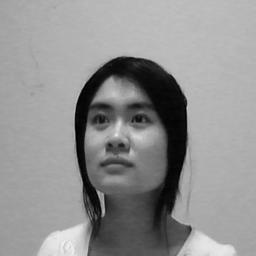
\includegraphics[width=2.5in]{sdumla_sample}
\caption{Amostra de imagem de SDUMLA-HTM após pré-processamento.}
\label{fig_sdumlahtm_sample}
\end{figure}

\subsection{Transformada Wavelet}
A extração de caracterísicas das imagens utilizou a transformada Wavelet. Esta técnica de processamento de sinal realiza a análise de um dado sinal no domínio do tempo e frequência \cite{costa2011ensemble}. Uma função Wavelet pode ser descrita como uma função que apresenta média zero e obedece a Equação:

\[\int_{-\infty}^{\infty} \Psi(t)dt = 0\]

Para utilizar a transformada Wavelet em imagens 2D as linhas e colunas são tratadas como sinais independentes. Ao final da decomposição Wavelet 2D são geradas 4 subimagens. Três delas (HL, LH, HH) contém os detalhes horizontais, verticais e diagonais da imagem original. Uma outra (LL) é uma aproximação da imagem original.

Ao final deste processo são gerados coeficientes que podem ser utilizados para representar a imagem original. Os coeficentes da imagem LL são geralmente os mais utilizados, pois apresentam menor dimensão e boa representatividade \cite{burrus1997introduction}.

\section{Classificadores}
Duas técnicas de aprendizado supervisionado foram implementadas para este trabalho: MLP e SVM. Estas técnicas não serão descritas em detalhe, pois já foram apresentadas em aula.

\subsection{MLP}
Multilayer Perceptron é um tipo de rede neural artificial feedforward. Neste trabalho, o treinamento das redes foi realizado utilizando a estratégia de backpropagation. O método do gradiente conjugado (de Polak-Ribière) foi o escolhido para otimizar os modelos, com a taxa de aprendizado definida pelo método de bisseção. Na seção \ref{sec:discussao} será mostrado que a utilização deste método permitiu acelerar a convergência dos treinamentos quando comparado à taxa de aprendizado fixa.

O critério de parada do treinamento da MLP foi dado pelo erro de validação. Esta estratégia reserva algumas amostras não utilizadas em treino, e computa o erro de validação destes dados a cada época. Quando o valor do erro de validação não diminuir por 5 épocas\footnote{Valor arbitrário, baseado em empirismo} seguidas, o treinamento é interrompido. Trata-se de uma estratégia para minimizar overfitting (pouca capacidade de generalização dos modelos).

MLPs são sensíveis à alta-dimensionalidade dos dados. Portanto, antes do treinamento foi necessário aplicar uma Análise de Componentes Principais (PCA) aos coeficientes obtidos da transformada Wavelet. Este procedimento selecionou um número de componentes de forma que a variância dos dados fosse pelo menos 90\%$^1$ do valor original. O resultado final definiu aproximadamente 70 valores para utilização no treinamento, variando de acordo da função wavelet, sub-bandas e nível de decomposição.

Uma das vantagens da MLP é o fato de lidar naturalmente com problemas multiclasses. Neste trabalho, dada uma imagem era necessário definir a qual dos N indivíduos ela pertence. Na rede neural isso se reflete com a existência de N neurônios na camada de saída, em que a ativação de cada um representa a identificação de um indivíduo.

%TODO: Inserir imagem mostrando erro de treino e validação
%TODO: Falar do ajuste de parâmetros: número de neurônio na camada oculta

\subsection{SVM}
Máquinas de Vetores Suporte são classificadores que efetuam a separação de amostras em um espaço, geralmente fazendo uso de uma função Kernel para realizar projeção de dados não linearmente separáveis no espaço original. Neste trabalho foi implementado o algoritmo Sequential Minimal Optimization (SMO), conforme visto em aula. 

Diferentemente da MLP, SVMs são insensíveis à alta-dimensionalidade e não necessitam do uso de PCA. Por outro lado, este algorítmo apresenta o problema de ser originalmente para classificação binária, portanto, foi necessário o uso de estratégia de classificação multi-classe, neste caso: One-vs-all. Neste método é preciso treinar um classificador para cada um dos N indivíduos, classificando-os em +1 (é o indivíduo) e -1 (não é o indivíduo). O critério de decisão foi dado pela maior distância da amostra ao hiperplano de separação.

Três tipos de função de kernel foram implementados para este trabalho: linear, gaussiano de base radial (rbf) e polinomial. Os parâmetros C, gamma e degree (grau do polinômio) foram ajustados durante o treinamento por meio de uma busca em grid e k-fold cross-validation.

\section{Avaliação}
A avaliação deste trabalho utilizou técnicas comuns à area de aprendizado de máquina: validação cruzada K-folds e um teste não paramétrico para comparação dos classificadores. As métricas utilizadas são: precisão, revocação e medida F1, adequadas à avaliação de problemas de classificação. Além disso, a métrica de acurácia foi utilizada na execução do teste não paramétrico, conforme será explicado na seção \ref{sec:friedman}.

\subsection{Validação cruzada K-folds}
Na validação cruzada K-folds\footnote{Em inglês, K-folds cross-validation} o conjunto de dados é dividido aleatoriamente em k subconjuntos de aproximadamente mesmo tamanho. O modelo é treinado com amostras de $k-1$ subconjuntos e validado no subconjunto não utilizado no treino (este processo se repete k vezes). A medida de acurácia dos modelos é obtida dividindo-se o número de classificações corretas de validação pelo total de amostras no conjunto de dados.

\subsection{Teste de Friedman} \label{sec:friedman}
O Teste de Friedman é um teste não paramétrico para comparar repetidas observações em mesmo objeto (ex: modelos computacionais) \cite{demvsar2006statistical,settouti2016statistical}. A estatística de Teste para Friedman é um $\chi^2$ com k-1 graus de liberdade. Quando o p-valor para este teste é pequeno ($< 0,05$), há evidência para rejeitar a hípótese nula. Para este trabalho, a hipótese nula declara que todos os modelos são equivalentes.

O método desse teste inicia-se a partir de uma matriz $X_{nxk}$, em que n é o número de conjuntos de teste, k é o número modelos computacionais, e cada elemento dessa matriz é um valor de acurácia para um modelo em um dos conjuntos. 

No segundo passo, calcula-se uma matriz $r_{nxk}$, que mostra o rank de um modelo para um dado conjunto (maior acurácia possui rank 1, segundo maior rank 2, e assim sucessivamente até o rank k). Os cálculos a seguir mostram como chegar à estatística de teste:

\[\overline{r_j} = \frac{1}{n} \sum_{i=1}^{n} r_{ij}\]

\[\overline{r} = \frac{1}{nk} \sum_{i=1}^{n} \sum_{j=1}^{k} r_{ij}\]

\[SS_t = n \sum_{j=1}^{k} \overline{r_j} - \overline{r}\]

\[SS_e = \frac{1}{n(k-1)} \sum_{i=1}^{n} \sum_{j=1}^{k} (\overline{r_{ij}} - \overline{r})^2\]

\[Q = \frac{SS_t}{SSe}\]

\begin{table}[!t]
\caption{Valores críticos para Teste de Friedman}
\label{table_friedman_values}
\centering
\begin{tabular}{|c|c|c|} \hline
& \multicolumn{2}{c|}{$k=3$} \\ \hline 
$n$&  0,05          &  0,01          \\ \hline
 2 &   -            &   -            \\
 3 & 6,000          &   -            \\
 4 & 6,500          & 8,000          \\
 5 & 6,400          & 8,400          \\
 6 & 7,000          & 9,000          \\
 7 & 7,143          & 8,857          \\
 8 & 6,250          & 9,000          \\
 9 & 6,222          & 9,556          \\
10 & \textbf{6,200} & \textbf{9,600} \\ \hline
\end{tabular}
\end{table}

A Tabela \ref{table_friedman_values} exibe os valores críticos de $Q$ para que a hipótese nula seja rejeitada.

\section{Experimento e Resultados} \label{sec:resultados}
Para gerar diferentes conjuntos de dados e acelerar o tempo de treinamento dos modelos as imagens de SDUMLA-HTM foram divididas em 10 conjuntos mutualmente exclusivos de 10 indivíduos.

Os resultados estão separados por função wavelet mãe (Daubechies e Symlets). Em todos os experimentos foi utilizado o nível de decomposição 3 e sub-banda LL, que produzem menor número de componentes e possuem boa representatividade \cite{burrus1997introduction}. 

Embora o kernel polinomial tenha sido implementado, resultados preliminares não foram satisfatórios. Assim o treinamento foi interrompido e os resultados não serão exibidos.

% O usuário deve definir três parâmetros, a saber:
% Nível de decomposição (1, 2 ou 3)
% Função wavelet mãe (db2, db4, sym3, sym4, sym5)
% Qual(is) sub-banda(s) utilizar (LL, HL, LH, HH)

\subsection{Daubechies}
A função db2 do MATLAB foi o wavelet da família Daubechies adotado para os resultados apresentados a seguir. A Tabela \ref{table_db2_rank} mostra o rank dos algoritmos SVM (kernel linear e RBF) e MLP nos 10 conjuntos de teste. Este rank é utilizado no teste não paramétrico, conforme explicado na seção \ref{sec:friedman}.
% TODO: Falar se o rank é diverso, se mostra indícios que um algoritmo é melhor

\begin{table}[!t]
\caption{Rank dos algoritmos SVM Linear, SVM RBF e MLP para coeficientes wavelet da família Daubechies}
\label{table_db2_rank}
\centering
\begin{tabular}{lccc}
\hline
Indivíduos & SVM Linear & SVM RBF & MLP \\
\hline
1-10   &  &  &  \\
11-20  &  &  &  \\
21-30  &  &  &  \\
31-40  &  &  &  \\
41-50  &  &  &  \\
51-60  &  &  &  \\
61-70  &  &  &  \\
71-80  &  &  &  \\
81-90  &  &  &  \\
91-100 &  &  &  \\ \hline
Média  &  &  &  \\
\end{tabular}
\end{table}

O valor da estatística de Friedman para estas medidas foi $Q = $, abaixo do valor crítico 6,2\footnote{Obtido da Tabela \ref{table_friedman_values}}. A seção \ref{sec:discussao} apresenta algumas considerações sobre este resultado.

Com o objetivo de ajudar a avaliar o desempenho dos modelos, precisão, revocação e medida-F1 são apresentadas na tabela \ref{table_db2_metric}. Para cada conjunto de teste é apresentada a média das 3 medidas para as 10 classes (indivíduos), além do valor médio para todos conjuntos.

\newpage
\subsection{Symlets}
A função sym5 do MATLAB foi o wavelet da família Symlets adotado para os resultados apresentados a seguir. A Tabela \ref{table_db2_rank} mostra o rank dos algoritmos SVM (kernel linear e RBF) e MLP nos 10 conjuntos de teste. Este rank é utilizado no teste não paramétrico, conforme explicado na seção \ref{sec:friedman}.
% TODO: Falar se o rank é diverso, se mostra indícios que um algoritmo é melhor

\begin{table}[!t]
\caption{Rank dos algoritmos SVM Linear, SVM RBF e MLP para coeficientes wavelet da família Symlets}
\label{table_sym5_rank}
\centering
\begin{tabular}{lccc}
\hline
Indivíduos & SVM Linear & SVM RBF & MLP \\
\hline
1-10   &  &  &  \\
11-20  &  &  &  \\
21-30  &  &  &  \\
31-40  &  &  &  \\
41-50  &  &  &  \\
51-60  &  &  &  \\
61-70  &  &  &  \\
71-80  &  &  &  \\
81-90  &  &  &  \\
91-100 &  &  &  \\ \hline
Média  &  &  &  \\
\end{tabular}
\end{table}

O valor da estatística de Friedman para estas medidas foi $Q = $, abaixo do valor crítico 6,2. A seção \ref{sec:discussao} apresenta algumas considerações sobre este resultado.

\begin{table*}[!t]
\caption{Precisão, revocação e medida F1 para coeficientes wavelet da família Daubechies}
\label{table_db2_metric}
\centering
\begin{tabular}{lccc|ccc|ccc} \hline
Indivíduos & \multicolumn{3}{c|}{SVM Linear} & \multicolumn{3}{c|}{SVM RBF} & \multicolumn{3}{c|}{MLP} \\ \hline
       & Precisão & Revocação & Medida-F1 & Precisão & Revocação & Medida-F1 & Precisão & Revocação & Medida-F1 \\ \hline
1-10   &   0,61   &   0,65    &   0,61    &   0,43   &   0,48    &   0,42    &   0,32   &   0,33    &   0,29    \\
11-20  &   0,53   &   0,60    &   0,53    &   0,39   &   0,46    &   0,39    &   0,01   &   0,08    &   0,02    \\
21-30  &   0,68   &   0,73    &   0,68    &   0,33   &   0,36    &   0,32    &   0,21   &   0,20    &   0,15    \\
31-40  &   0,50   &   0,55    &   0,50    &   0,42   &   0,46    &   0,41    &   0,40   &   0,42    &   0,47    \\
41-50  &   0,40   &   0,48    &   0,41    &   0,13   &   0,20    &   0,14    &   0,03   &   0,11    &   0,04    \\
51-60  &   0,11   &   0,20    &   0,12    &   0,01   &   0,11    &   0,02    &   0,13   &   0,21    &   0,14    \\
61-70  &          &           &           &          &           &           &          &           &           \\
71-80  &          &           &           &          &           &           &          &           &           \\
81-90  &          &           &           &          &           &           &          &           &           \\
91-100 &          &           &           &          &           &           &          &           &           \\ \hline
Média  &          &           &           &          &           &           &          &           &           \\
\end{tabular}
\end{table*}


\begin{table*}[!t]
\caption{Precisão, revocação e medida F1 para coeficientes wavelet da família Symlets}
\label{table_db2_metric}
\centering
\begin{tabular}{lccc|ccc|ccc} \hline
Indivíduos & \multicolumn{3}{c|}{SVM Linear} & \multicolumn{3}{c|}{SVM RBF} & \multicolumn{3}{c|}{MLP} \\ \hline
       & Precisão & Revocação & Medida-F1 & Precisão & Revocação & Medida-F1 & Precisão & Revocação & Medida-F1 \\ \hline
1-10   &   0,72   &   0,78    &   0,73    &   0,30   &   0,37    &   0,30    &   0,18   &   0,22    &   0,19    \\
11-20  &   0,64   &   0,66    &   0,62    &   0,32   &   0,36    &   0,30    &   0,30   &   0,35    &   0,29    \\
21-30  &   0,80   &   0,83    &   0,80    &   0,41   &   0,40    &   0,37    &   0,00   &   0,07    &   0,01    \\
31-40  &   0,62   &   0,62    &   0,60    &   0,32   &   0,37    &   0,32    &   0,19   &   0,29    &   0,21    \\
41-50  &   0,44   &   0,47    &   0,42    &   0,24   &   0,31    &   0,24    &   0,34   &   0,33    &   0,28    \\
51-60  &   0,01   &   0,08    &   0,01    &   0,09   &   0,16    &   0,09    &   0,38   &   0,38    &   0,36    \\
61-70  &          &           &           &          &           &           &          &           &           \\
71-80  &          &           &           &          &           &           &          &           &           \\
81-90  &          &           &           &          &           &           &          &           &           \\
91-100 &          &           &           &          &           &           &          &           &           \\ \hline
Média  &          &           &           &          &           &           &          &           &           \\
\end{tabular}
\end{table*}

\newpage

\section{Discussão} \label{sec:discussao}

Os resultados exibidos na seção \ref{sec:resultados} mostram que, em geral, as implementações dos algoritmos SVM e MLP não apresentaram bom desempenho. O algoritmo que obteve melhores resultados foi o SVM de kernel linear, que consistentemente obteve precisão, revocação e medida-F1 superior aos outros algoritmos.

A diferença entre os resultados do SVM Linear e SVM RBF possivelmente deve-se ao fato deste último depender do ajuste de mais parâmetros (C e gamma) que o primeiro (C). O kernel RBF é sensível a escolha do gamma, e este foi testado com valores muito baixos ~(1/número de componentes). Esta escolha pretendia diminuir o \textit{bias} do modelo, no entanto pode ter causado aumento da variância.

O mau desempenho da MLP pode ter relação com a decisão de adicionar tempo de processamento como um dos critério de parada. Resultados preliminares mostraram que utilizar apenas erro de validação como critério de parada tornaria o treinamento inviável para o hardware e tempo disponíveis. Uma alternativas pensadas foi implementar o método do gradiente conjugado de Polak-Ribière para otimizar o passo, porém não foi suficiente para diminuir o tempo de treinamento. 

%\begin{figure}[!t]
%\centering
%\includegraphics[width=2.5in]{myfigure}
%\caption{Simulation results for the network.}
%\label{fig_sim}
%\end{figure}

%\begin{figure*}[!t]
%\centering
%\subfloat[Case I]{\includegraphics[width=2.5in]{box}%
%\label{fig_first_case}}
%\hfil
%\subfloat[Case II]{\includegraphics[width=2.5in]{box}%
%\label{fig_second_case}}
%\caption{Simulation results for the network.}
%\label{fig_sim}
%\end{figure*}

%\begin{table}[!t]
%% increase table row spacing, adjust to taste
%\renewcommand{\arraystretch}{1.3}
%\caption{An Example of a Table}
%\label{table_example}
%\centering
%\begin{tabular}{|c||c|}
%\hline
%One & Two\\
%\hline
%Three & Four\\
%\hline
%\end{tabular}
%\end{table}

\bibliographystyle{IEEEtran}
\bibliography{bare_conf}

\end{document}